\clearpage
\section{删掉点光源后分簇绘制中断}

在一块金属面板前放三盏灯，逐灯绘制和分簇绘制都能看见同一个高光。接着删掉两盏，在余下那盏与面板之间放一个立方体，原本要检查两种算法能不能得到同一块阴影。可分簇绘制还没开始着色，就报出 \texttt{Upload must cover the complete compute resource}。此时连遮挡用的射线都没有发出。

点光源的记录占 32 个字节，前一组数保存位置，后一组保存红绿蓝强度和照明半径。三盏灯相当于 96 字节，剩下一盏只有 32 字节。Vulkan 的这个上传入口每次替换整份缓冲区。原来的调用只在灯数增加时换缓冲区，于是删灯后试图把 32 字节交给仍有 96 字节的目标。下面摘出决定大小的那行 C++。

\begin{Code}
// ScreenEffects.cpp, DrawLights: original allocation condition.
if (count > LightCapacity)
    Lights = Device.CreateBuffer(count * sizeof(GILight));
\end{Code}

改成 \texttt{count != LightCapacity} 后，增加灯和减少灯都会按实际长度重建。没有灯时仍保留最小的可绑定资源，传给着色器的灯数为零。无需放宽底层上传的约定，也不必每帧重新分配。GPU 用完的旧资源由现有计算设备管理。

\begin{center}

\includegraphics[width=.30\linewidth]{../../../output/profiling/point-materials/rough-metal.png}\hspace{8mm}
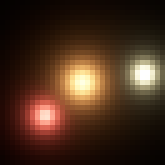
\includegraphics[width=.30\linewidth]{../../../output/profiling/point-materials/smooth-metal.png}\\
{\small 测试中的同一块面板。三盏灯下，粗糙度从 0.70 调到 0.25，高光集中。}
\end{center}

复测在同一个 \texttt{ScreenEffects} 对象上先算三盏灯，再换成一盏被遮住的灯。两种算法读到的面板中心 RGB 都是零，程序能继续绘制。三灯时另外核对了整幅图；RenderDoc 事件 8 与 33 在光滑面板中心都读到约 $(16.105,5.636,1.450)$。从仓库根目录运行下面的批处理可以复现。\href{run:../../tests/PointMaterialCheck.h}{测试源码}\quad\href{run:../profiling/point-materials/renderdoc.json}{RenderDoc 读数}

\begin{Code}
REM Run from the repository root. Compare three lights, then one.
tests\run_screen_effects.cmd --point-materials
\end{Code}
